% Especificaciones del tamaño de letra, tamaño de hoja, márgenes, librerias, etc.
\documentclass[letterpaper]{article}
\usepackage[english]{babel}
\usepackage[utf8]{inputenc}
\usepackage[T1]{fontenc}
\usepackage{mathrsfs}
\usepackage{amsmath}
\usepackage{graphicx}
\usepackage{subcaption}
\usepackage{hyperref}
\usepackage{url}
\usepackage{amssymb}
\usepackage{float}
\usepackage[framed, numbered]{matlab-prettifier}
%\usepackage[framed, numbered, autolinebreaks, useliterate]{mcode}
\usepackage[margin=1in]{geometry}
\renewcommand{\baselinestretch}{1}

% Enlace Bibliografía
\usepackage{csquotes}
\usepackage[notes,backend=biber]{biblatex-chicago}
\addbibresource{referencias.bib}

% Titulo, autores, fecha.
\title{Tarea \#3: Función de Transferencia}
\author{Carlos Vásquez 1155057}

% Inicio del documento
\begin{document}
\maketitle
\subsection*{Resolver:}
Obtener la función de transferencia, asumiendo que $\mu \neq 0$, que relaciona la función $x_1(t)$ ante la entrada $u(t)$ del sistema que se muestra a continuación.
\begin{figure}[H]
	\centering
	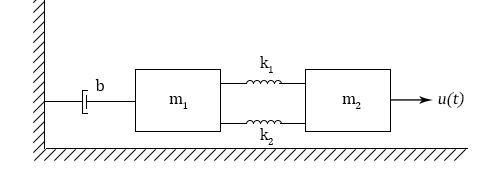
\includegraphics[width=0.5\textwidth]{sys.png}
	\caption{Sistema a analizar.}
\end{figure}
\textbf{Solución}

Analizando el sistema, podemos obtener las siguientes ecuaciones que lo rigen:
\begin{equation}
	\begin{split}
		0 &= m_1 \ddot x_1 + (\mu_1 + b)\dot x_1 + (k_1 + k_2)x_1 - (k_1 + k_2)x_2 \\
		u(t) &= m_2 \ddot x_2 + \mu_2 \dot x + (k_1 + k_2)x_2 - (k_1 + k_2)x_1
	\end{split}
\end{equation}

Aplicando la transformada de Laplace obtendremos el siguiente sistema en el espacio s:

\begin{equation}
	\begin{split}
		0 &= M_1 s^2 X_1(s) + (\mu_1 + B)s X_1(s) + (k_1 + k_2)X_1(s) - (k_1 + k_2)X_2(s) \\
		U(s) &= M_2 s^2 X_2(s) + \mu_2 sX_2(s) + (k_1 + k_2)X_2(s) - (k_1 + k_2)X_1(s)
	\end{split}
\end{equation}

Posteriormente, del sistema de ecuaciones (2) despejamos a $X_2(s)$
\begin{equation}
	X_2(s) = \frac{X_1(s)(M_1 s^2 + (\mu_1 + B)s + k_1 + k_2)}{k_1 + k_2}
\end{equation}

Sustituyendo la ecuación (3) en el sistema (2) obtenemos
\begin{equation}
	U(s) = X_1(s) \left(  \frac{(M_2s^2 + \mu_2s + (k_1 + k_2))(M_1s^2 + (\mu_1 + B)s + k_1 + k_2)}{k_1 + k_2} - (k_1 + k_2) \right)
\end{equation}

Simplificando la ecuación 4 y despejando para encontrar $\frac{X_1(s)}{U(s)}$
\begin{equation}
	\boxed{\frac{X_1(s)}{U(s)} = \frac{k_1 + k_2}{(M_1s^2 + (\mu_1 + B)s + k_1 + k_2)(M_2s^2 + \mu_2s + k_1 + k_2) - (k_1 + k_2)^2}}
\end{equation}
%%%%% Bib
\renewcommand\refname{Referencias}
\printbibliography
\end{document}
